\cotefile{156-9}
\scanpage{2}
% archive sheet number: 1
% top right
\hfill GF \uline{$\overline{\mathrm{IX}}$}

\margin{(voir p \unsure{75} la mise au pt sur la terminologie\unsure{)}}

\diagram{%
\begin{tikzcd}[ampersand replacement=\&,column sep=small,row sep=large,execute at end picture={\draw[gray,line width=1.2pt] (sepA.center)--(sepB.center);}]
\& \& \begin{gathered}\text{Atelier général}\quad\text{\textcircled{$\unsure{\mathscr A|\mathcal A}$}}\\(\mathscr A,\unsure{\unlhd|\trianglelefteq},\ll,|\circ|)\end{gathered}
 \arrow[dll,dash] \arrow[dl,dash] \arrow[dr,dash] \arrow[drr,dash] \arrow[dddrr,bend left=35] \& \& \\
\begin{gathered}\text{\uline{atelier spatial}}\\(\mathscr A_{\unsure{\varphi}},\unlhd,|\circ|)\quad\text{\textcircled{$\Sigma$}}\end{gathered}
 \arrow[dr,dash] \arrow[ddrr] \arrow[dddrrr,dashed,dash]
 \& \begin{gathered}\text{\deleted{\uline{\unsure{Atlier|Atelier} divisé}}}\\\text{\uline{atelier local}}\\(\mathscr A,\unlhd,\ll,|\circ|_{\unsure{\ll}})\end{gathered}\arrow[d,dash]
 \& \& \begin{gathered}\text{\uline{atelier fidèle}}\\(\mathscr A,\unlhd,\ll)\end{gathered}\arrow[dll,dash]\arrow[ddd]
 \& \text{\deleted{atelier modéré}}\\
\& \begin{gathered}\text{\uline{atelier ponctuel}}\\\Sigma\simeq\unsure{\mathscr P|\mathcal P}(2)\end{gathered}\arrow[dr]\arrow[rr,dashed,dash,bend right=30,"?"']
 \& \& \text{\uline{at. mod}\ ?} \& \\
\& \& \begin{gathered}\text{\textcircled{$\unsure{\mathscr L|\mathcal L}$}}\ \text{\uline{atelier ensembliste}}\end{gathered}\arrow[d]
 \& \& \text{atelier modéré}\arrow[dl]\arrow[dll,dashed]\\
\& \& \text{\uline{at. ens. modéré}}\arrow[dd]
 \& \begin{gathered}\text{maquette}\ \Sigma\simeq\mathscr P(\mathscr A)\end{gathered}\arrow[ddl] \& \\
|[alias=sepA]|{} \& \& \& \& |[alias=sepB]|{} \\
\& \& \text{at. \uline{discret}}\arrow[d]\& \& \\
\& \& \begin{gathered}\text{\deleted{\unsure{at. final}}}\\\text{\uline{at.-point}}\end{gathered}\& \&
\end{tikzcd}}
\margin{\figure{\begin{tikzpicture}
\node[anchor=north west,inner sep=1pt,text width=\marginparwidth,align=left] (note) at (0,0) {\uline{NB} Si les ateliers mod sont fidèles, le diagramme se simplifie \unsure{at mod se place} entre at fid et maq.};
\draw[gray] ([xshift=-2mm,yshift=2mm]note.north west) .. controls ([xshift=8mm,yshift=3mm]note.north west) and ([xshift=-6mm,yshift=3mm]note.north east) .. ([xshift=2mm,yshift=0mm]note.north east) -- ([xshift=2mm,yshift=-2mm]note.south east) .. controls ([xshift=-6mm,yshift=-2mm]note.south east) and ([xshift=6mm,yshift=-2mm]note.south west) .. ([xshift=-2mm,yshift=-2mm]note.south west);
\end{tikzpicture}}}

Je \unsure{me suis intéressé} plus particulièrement \inserted{\unsure{donc}} \unsure{par|pour} les ateliers \uline{spatiaux} \inserted{(Si on \unsure{veut}!)}, incluant les ateliers ensemblistes, comme ceux définis par des \deleted{\unsure{ens. ord.}} ``ensembles ordonnés'', et les maquettes. (at. sp. \unsure{locaux}).

Parmi ceux-ci, pour un travail \inserted{\unsure{primaire} par certains côtés,} proche de l'\unsure{impact} de la topologie ensembliste, je suis intéressé par les ateliers qui sont de plus locaux. (Cela exclut les maquettes, parmi les exemples précédents, sauf les maquettes discrètes).

En développant \unsure{d'abord} une topologie modérée, je m'intéresserai aux \uline{ateliers modérés} (\unsure{ensemblistes} ou non) -- qui incluent les maquettes. Je présume qu'il y a lieu \deleted{\unsure{de s'imposer}} pour les ateliers modérés \deleted{\unsure{qu'ils soient}} \inserted{d'être \uline{\unsure{spatiaux}} (\unsure{voire} pas néc. locaux)}, et peut être
% stamp: TSUP
